\chapter[General Project Framework and Methodology]{General Project Framework \\ and Methodology}

\section{Introduction}
To establish a clear, academically rigorous roadmap for the design, development, and realization of the \textbf{Predictra Threat Map}, it is essential to first understand the organizational environment, project context, and state of the art in the threat intelligence domain. This chapter introduces our host company, details the commercial and open-source landscape of Cyber Threat Intelligence (CTI) platforms, critiques existing market solutions, and defines the Agile Scrum framework and UML standards adopted as our development and modeling methodologies.

\section{Host Organization: Predictra}

\subsection{Company Profile and Mission}
This graduation project was hosted by \textbf{Predictra}, a next-generation cybersecurity technology firm specializing in AI-driven Cyber Threat Intelligence (CTI). Predictra's core vision is to democratize threat intelligence, converting millions of raw, distributed cybersecurity data points into highly structured, real-time, and visually actionable insights. 

Predictra provides enterprise security teams, Security Operations Centers (SOCs), and threat researchers with advanced reconnaissance capabilities, brand monitoring, ransomware leak tracking, and infrastructure threat analysis. The host company represents a modern threat-focused corporate environment, providing access to massive telemetry datasets and industrial expertise in cyber adversary tracking.

Predictra's platforms leverage advanced machine learning models to ingest unstructured data from public channels, dark web marketplaces, chat platforms, and open-source repositories. The goal of the organization is to equip modern security departments with proactive defenses, shifting the security paradigm from reactive incident response to predictive threat preemption. By offering real-time visibility into adversary activities, Predictra empowers companies to actively block threats before they breach internal network perimeters.

\subsection{Organizational Structure}
To support its mission of providing real-time global intelligence, Predictra is structured into three highly specialized departments, as modeled in Figure~\ref{fig:predictra_org}.

\begin{figure}[H]
\centering
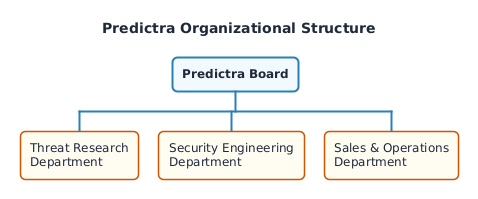
\includegraphics[width=0.9\textwidth]{assets/predictra_org.png}
\caption{Organizational structure of Predictra.}
\label{fig:predictra_org}
\end{figure}

The specific responsibilities of these departments are detailed below:
\begin{itemize}
    \item \textbf{Threat Research Department:} Composed of security analysts and researchers. This department focuses on analyzing cyber campaigns, monitoring extortion websites, and maintaining threat databases. They validate threat indicators and create signatures. Their operations involve examining malware samples, tracking attacker networks, and cataloging actor tactics. Their output is threat intelligence used to feed the ingestion platforms.
    \item \textbf{Security Engineering Department:} Composed of software and database developers. This department is responsible for building ingestion pipelines, data streaming, and the user interface. They focus on database performance, user experience, and cloud deployments. They coordinate with researchers to support new threat indicators.
    \item \textbf{Sales and Operations Department:} Manages client relations, enterprise deployments, marketing campaigns, and commercial threat briefing dissemination, ensuring the platform's features align with commercial market requirements. They gather user feedback from enterprise customers, identify market gaps, and coordinate training and technical support services.
\end{itemize}

\subsection{Inter-Departmental Workflows}
To maintain a high velocity of threat detection and update dissemination, these three departments coordinate via highly structured workflows. When the Threat Research team identifies a new ransomware leak site or an active botnet command-and-control server cluster, they compile the technical signatures and pass them to the Security Engineering team. 

The engineers design new scrapers or update the existing classification databases to support these indicators. Once validated, the engineering team deploys the updates to production environments. Finally, the Sales and Operations team briefs enterprise clients on the newly integrated monitoring capabilities, gathering immediate operational feedback to guide future development iterations.

\section{Project Context and Problem Definition}

Historically, analyzing external threat feeds was a slow, manual process. Threat intelligence teams had to poll separate tabular feeds, manually normalize indicators, and compile static briefings. This tabular approach creates a high **compromise dwell time** -- often exceeding 200 days -- during which adversaries move laterally undetected. Furthermore, Security Operations Center (SOC) analysts suffer from visual fatigue when looking at thousands of static text logs in spreadsheets or simple dashboards. They lack an intuitive, real-time spatial visual interface that provides immediate, global threat situational awareness at a glance.

The \textbf{Predictra Threat Map} was conceived to bridge this critical operational gap, transforming high-velocity, multi-source external cyber threat data into a live, interactive, 3D visual intelligence map and structured analysis dashboard.

\section{State of the Art: Comparative Analysis of CTI Solutions}
To design a robust CTI platform, we conducted a rigorous comparative analysis of existing open-source and commercial threat intelligence solutions, evaluating their data models, stream latencies, spatial visualization support, and hardware footprints.

\subsection{Open-Source Solutions}

\subsubsection{MISP (Malware Information Sharing Platform)}
MISP is a widely used open-source platform for sharing threat information. It supports storing and tagging IP addresses, file hashes, and domains.

From a technical perspective, MISP uses standard database structures. While it is highly capable at storing large lists of historical threats, it is not optimized for real-time streaming. Analysts must request updates periodically, which introduces delays. Furthermore, the user interface consists primarily of text-based tables and lacks real-time 3D visual maps.

Maintaining a MISP instance requires regular management. Security teams must allocate engineering resources to monitor the system and refine database rules. Additionally, because the interface is complex, security teams must spend time training analysts before using it in security operations.

\subsubsection{OpenCTI (Open Cyber Threat Intelligence)}
OpenCTI is a modular platform designed to represent threat intelligence as a graph, linking actors, campaigns, malware, and targeted sectors. It uses specialized databases for indexing and searching, and features connectors to import public and private threat feeds.

However, OpenCTI's architecture is heavy. Running the platform requires managing multiple service layers, which demands high-specification servers and increases operational costs. Furthermore, the interface is optimized for long-term analytical research rather than real-time visual tracking.

From a hosting perspective, the server requirements mean that organizations must allocate significant hardware resources. For smaller teams, this makes the hosting costs high, reducing the financial benefits of using open-source software.

\subsection{Commercial Solutions}

\subsubsection{Recorded Future}
Recorded Future is a major commercial platform that gathers threat indicators from web, forum, and social media channels. It translates these pages into standardized profiles, offering threat scoring and technical indicators, with integrations for major security tools.

Despite its capabilities, Recorded Future is highly expensive, making it inaccessible to smaller organizations. Furthermore, the dashboard is focused on text reports and simple static 2D maps, lacking real-time animations for display screens.

Because it is a closed system, organizations must rely entirely on the vendor's algorithms. Integrating custom data sources not supported by default can be difficult and costly.

\subsubsection{Cyble}
Cyble is a commercial provider focusing on brand protection and monitoring online forums and chat channels for leaked credentials and assets. It provides automated alerts and risk indicators.

Like other commercial options, Cyble requires subscription fees and does not allow custom developer integrations. Its interfaces are designed as static reports, lacking real-time animations, which limits its usefulness for active display environments.

\subsection{Comparative Summary Table}
To clarify the distinctions, a comparative matrix of key platform parameters is detailed in Table~\ref{tab:cti_comparison}.

\begin{table}[H]
\centering
\small
\arrayrulecolor{charcoal!30}
\rowcolors{2}{cyberblue!5}{white}
\begin{tabularx}{\textwidth}{>{\raggedright\arraybackslash}p{2.8cm}XXXX}
\hline
\rowcolor{charcoal}
\thc{Feature / Metric} & \thc{MISP} & \thc{OpenCTI} & \thc{Recorded Future} & \thc{Predictra Threat Map} \\
\hline
Data Model & Attributes / Events & STIX 2.1 Graph~\cite{stix_specification} & Proprietary Graph & Hybrid (SSE + STIX 2.1) \\
Real-Time Streaming & Low (Sync APIs) & Medium (API Poll) & Medium & High (300ms SSE Flush) \\
Visual Spatial Mapping & None & None & Limited 2D Maps & 3D WebGL Globe \& 2D \\
System Resource Footprint & Medium & Very High & N/A (SaaS) & Low (Optimized Node/React) \\
Target Audience & Incident Responders & Intel Analysts & Enterprise SOCs & Modern SOCs \& SMEs \\
Financial Accessibility & Free / Open Source & Free / Open Source & Highly Prohibitive & Open and Accessible \\
\hline
\end{tabularx}
\caption{Academic comparative analysis of global CTI solutions.}
\label{tab:cti_comparison}
\end{table}

\section{Critique of Existing Systems and Proposed Solution}
The evaluation of the state of the art highlights a clear market gap: \textbf{existing CTI platforms are either highly analytical but visually static and resource-heavy (like OpenCTI and MISP), or visually polished but commercially restrictive (like Recorded Future)}. 

To resolve this gap, we proposed the \textbf{Predictra Threat Map}. Our solution is designed as a real-time threat visualizer and analysis workspace:
\begin{itemize}
    \item It uses a modular scraper architecture fetching data from 9+ feeds. This ensures resilience, as the failure of one external feed does not affect others.
    \item It streams events instantly using a coordinated batching queue, keeping browser load low and ensuring smooth data delivery.
    \item It displays an interactive 3D virtual Earth, visualizing threat locations as dynamic curved paths using hardware acceleration.
    \item It integrates a client-side STIX 2.1 file parser, providing analysis features directly in the browser without requiring complex databases.
\end{itemize}

By separating backend data ingestion from frontend visualization and optimizing client-side math, the platform provides high-quality graphics and analysis without requiring expensive server clusters.

\section{Work Methodology and Modeling Standards}
To ensure the rigorous and efficient delivery of this software platform, the project adopted standard industry methodologies for development and system modeling.

\subsection{Agile Scrum Framework}
We implemented the \textbf{Agile Scrum framework} to pilot the development process. This methodology split the project lifecycle into iterative, fully functional increments called \textbf{Sprints}.

\begin{figure}[H]
\centering
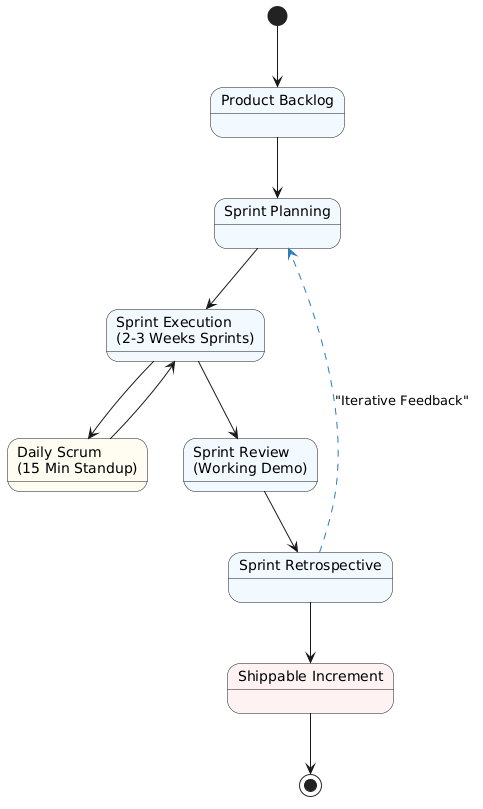
\includegraphics[width=0.8\textwidth]{assets/scrum_lifecycle.png}
\caption{Agile Scrum development lifecycle flowchart.}
\label{fig:scrum_lifecycle}
\end{figure}

The Scrum lifecycle details are structured as follows:
\begin{itemize}
    \item \textbf{Roles:} Brahim Jaballi and Chiheb Amri shared the developer role, with Chiheb coordinating scrum master tasks (sprint planning, daily standups, backlog refinement) and industrial mentors acting as the Product Owner.
    \item \textbf{Sprint Planning (Duration: 2 Hours):} Held at the start of each sprint. The team analyzed the Product Backlog, estimated task complexities using Planning Poker (Fibonacci scale), and committed to a Sprint Backlog. This ritual ensured that the team maintained a clear, realistic set of deliverables for each iteration, avoiding scope creep. Task complexity was evaluated relative to standard reference cards, helping to identify potential design bottlenecks early.
    \item \textbf{Sprint Execution (Duration: 2-3 Weeks):} Active coding, database design, visual design, and integration testing of the committed backlog items. The work was divided using git branch collaborations. The team used continuous integration strategies to ensure that the code on the main branch compiled flawlessly at the end of each day.
    \item \textbf{Daily Scrum (Duration: 15 Minutes):} A daily morning meeting where both team members aligned by answering: What was done yesterday? What will be done today? What are the blockers? This ceremony kept the development highly coordinated and immediately resolved technical bottlenecks, such as library version conflicts or database access permissions.
    \item \textbf{Twice-Weekly Coordination and Review Meetings:} Extended coordination sessions held specifically on Thursdays and Sundays to handle deep code integration, performance profiling, and strategic sprint planning (detailed in Subsection~\ref{subsec:biweekly_meetings}).
    \item \textbf{Sprint Review (Duration: 1.5 Hours):} Conducted at the end of each sprint. The developers demonstrated a working system increment (e.g., the Scraper Pipeline in Sprint 1, the WebGL Globe in Sprint 2) to obtain Product Owner feedback and validate user stories. Any feedback or modification requests were immediately converted into new backlog items.
    \item \textbf{Sprint Retrospective (Duration: 1 Hour):} Held immediately after the review, where the team identified engineering process bottlenecks (e.g. testing bottlenecks, git merge conflicts) and defined continuous improvement action items. This ceremony ensured that team performance improved incrementally with each sprint.
\end{itemize}

\subsection{Twice-Weekly Scrum Coordination and Technical Review Rituals}
\label{subsec:biweekly_meetings}
Because the development of the \textbf{Predictra Threat Map} involved both high-throughput distributed database ingestion systems (scrapers, BSON caches, geocoding) and complex browser-side WebGL canvas renderers, standard 15-minute Daily Scrum meetings were insufficient to resolve dense architectural alignment and integration bottlenecks. To address this, the development team (Brahim Jaballi and Chiheb Amri) instituted an additional twice-weekly extended coordination and technical review cadence, occurring without fail every Thursday and Sunday over the entire six-month project lifecycle (representing over 48 intensive sessions in total).

These bi-weekly sessions acted as the technical anchors of the project. They ensured that both developer branches remained continuously integrated and that any performance bottlenecks (such as garbage collection spikes or memory leaks in the Three.js render loop) were diagnosed and resolved immediately.

\subsubsection{Thursday Technical Alignment Sessions}
The Thursday meetings, typically lasting 3 hours, were positioned at the mid-point of each sprint. Their core purpose was to ensure technical alignment, verify code compilation, and perform peer code reviews. The agenda and operational details are structured below:
\begin{itemize}
    \item \textbf{Code Review and Pull Request Merging:} The developers conducted line-by-line peer reviews of newly written features (e.g., a new scraper module or a UI widget). Branch merges into the local \texttt{develop} environment were executed during this session.
    \item \textbf{API Schema Verification:} External threat intelligence feeds (such as AlienVault OTX or URLhaus) frequently update their JSON fields without notice. Thursdays were used to audit incoming API payloads against our local Mongoose database schemas, resolving any mapping errors or missing geocoding fields.
    \item \textbf{Performance Profiling Sandbox:} Developers ran Chrome DevTools profiling sessions on the rendering thread, checking that the addition of new visual elements (like animated great-circle arcs) did not degrade the rendering framerate below 60fps.
\end{itemize}

\subsubsection{Sunday Strategic Integration and Planning Sessions}
The Sunday meetings, typically lasting 4 hours, were conducted at the end of each weekly cycle. These sessions focused on architectural consolidation, long-term technical planning, and product owner briefings. Their core agenda included:
\begin{itemize}
    \item \textbf{End-of-Week Architectural Refactoring:} Over the course of weekly active coding, developers often introduced minor technical debt. Sundays were dedicated to refactoring complex components, consolidating Zustand store states, cleaning CSS variables, and auditing TypeScript type safety.
    \item \textbf{Academic Documentation Consolidation:} To maintain a high-quality graduation thesis, the team spent the last hour of every Sunday session documenting the technical achievements, designing UML diagrams, and updating the LaTeX report to reflect the current sprint's results.
    \item \textbf{Next-Sprint Planning and Backlog Commitment:} In alignment with upcoming milestones, developers refined the backlog, estimated task sizing using Planning Poker, and committed to the deliverables for the subsequent weekly cycle.
\end{itemize}

To summarize, the operational structure of these twice-weekly coordination sessions is detailed in Table~\ref{tab:biweekly_meetings}.

\begin{table}[H]
\centering
\small
\arrayrulecolor{charcoal!30}
\rowcolors{2}{cyberblue!5}{white}
\begin{tabularx}{\textwidth}{>{\raggedright\arraybackslash}p{2.3cm}XX}
\hline
\rowcolor{charcoal}
\thc{Parameter} & \thc{Thursday Technical Alignment} & \thc{Sunday Strategic Integration} \\
\hline
\textbf{Session Focus} & Technical Integration, Code Auditing, Bug Diagnostics & Architectural Consolidation, Documentation, Sprint Planning \\
\textbf{Typical Duration} & 3.0 Hours & 4.0 Hours \\
\textbf{Key Inputs} & Local Feature Branches, Scraper Output Logs, Performance Metrics & Consolidated \texttt{develop} Branch, Open Backlog, Academic Guide \\
\textbf{Key Activities} & Peer reviews, API schema validation, WebGL frame profiling, branch merging & Code refactoring, Zustand state pruning, LaTeX documentation, backlog sizing \\
\textbf{Primary Output} & Integrated, stable mid-sprint code build & Cleaned production build, updated UML blueprints, next sprint backlog \\
\textbf{Lifespan Coverage} & Every week over 6-month duration (48+ sessions) & Every week over 6-month duration (48+ sessions) \\
\hline
\end{tabularx}
\caption{Operational breakdown of bi-weekly coordination meetings held over 6 months.}
\label{tab:biweekly_meetings}
\end{table}

\subsection{UML Modeling Standards}
To guarantee a solid architectural design, the system requirements, conception, and structure were modeled utilizing the \textbf{Unified Modeling Language (UML)}.
\begin{itemize}
    \item \textbf{Use Case Diagrams:} Captured functional system boundaries and actor-system boundaries. They helped define what services the system must deliver and which human or external actors trigger them, providing a clear map of system responsibilities.
    \item \textbf{Class Diagrams:} Modeled Mongoose database schemas, backend services, and Zustands stores, laying out the structural blueprints of our classes, variables, and methods. These diagrams were crucial in establishing a type-safe structure during TypeScript integrations.
    \item \textbf{Sequence Diagrams:} Traced asynchronous communication timelines between analysts, backend event streams, and front-end render loops, verifying transaction safety and identifying potential race conditions or connection deadlocks.
    \item \textbf{Component Diagrams:} Illustrated modular package boundaries and code dependencies, ensuring a decoupled physical architecture that facilitates scaling.
\end{itemize}

\section{Conclusion}
This chapter established the academic, professional, and methodological foundations of our project. Having analyzed the CTI domain, compared existing market solutions, and set up our Scrum and UML modeling structures, we proceed to Chapter 2 to detail the requirements, project preparation, sprint planning, and the global architecture of the Predictra CTI platform.
